\subsection{Two electrons in two dimensions}

\subsubsection{Brute force sampling}

Standard error of the mean (SEM):
\begin{equation}
\text{SEM} = \frac{\sigma}{\sqrt{N}}
\end{equation}
where $N$ is the number of observations, in our case the number of Monte Carlo cycles.

\begin{table}[H]\caption{Comparing the results for analytical/numerical evaluation of the double derivative. Energy are in atomic units (a.u.) and CPU time is in units of seconds. Number of MC cycles are 2$^{21}$.}\label{tab:brute_force_no_interaction_2p}
\center
\begin{tabular}{l|l}
Analytical: &  Numerical:\\ \hline
\begin{tabular}{ccccc}
$\alpha$: & $\left< E_L \right>$: & SEM: & $\sigma_B$: & CPU time:\\ \hline
0.50 & 2.49402 & 0.00073 & 0.01022 & 5.57812\\
0.60 & 2.26441 & 0.00052 & 0.00690 & 5.76562\\
0.70 & 2.13118 & 0.00035 & 0.00448 & 5.92188\\
0.80 & 2.05016 & 0.00022 & 0.00263 & 5.67188\\
0.90 & 2.01015 & 0.00010 & 0.00116 & 5.96875\\
1.00 & 2.00000 & 0.00000 & 0.00000 & 5.62500\\
1.10 & 2.00871 & 0.00009 & 0.00102 & 6.20312\\
1.20 & 2.03402 & 0.00018 & 0.00175 & 6.34375\\
1.30 & 2.07259 & 0.00026 & 0.00244 & 5.95312\\
1.40 & 2.11041 & 0.00034 & 0.00311 & 6.15625\\ \hline
\end{tabular} & \begin{tabular}{ccccc}
$\alpha$: & $\left< E_L \right>$: & SEM: & $\sigma_B$: & CPU time:\\ \hline
0.50 & 2.49991 & 0.00073 & 0.01093 & 18.20310\\
0.60 & 2.26412 & 0.00053 & 0.00727 & 18.21880\\
0.70 & 2.13039 & 0.00036 & 0.00436 & 18.62500\\
0.80 & 2.04993 & 0.00022 & 0.00269 & 18.46880\\
0.90 & 2.01160 & 0.00010 & 0.00118 & 18.46880\\
1.00 & 2.00000 & 0.00000 & 0.00000 & 18.31250\\
1.10 & 2.00825 & 0.00009 & 0.00097 & 18.35940\\
1.20 & 2.03308 & 0.00018 & 0.00170 & 18.31250\\
1.30 & 2.06460 & 0.00026 & 0.00243 & 20.23440\\
1.40 & 2.11803 & 0.00033 & 0.00308 & 19.00000\\ \hline
\end{tabular}\\
Mean CPU time: 5.91875 & Mean CPU time:  18.62033\\
\end{tabular}
\end{table}

\subsubsection{Including importance sampling}

Figure \ref{fig:comparing_sampling} compare the expectation value of the energy and the acceptance rate of brute force sampling and importance sampling. It can be observed from the right part of the figure that the acceptance rate of both methods increase with decreasing step size, but one can also observe that the acceptance is lower for importance sampling than brute force sampling at large step sizes. These observations could indicate that a small step size would be ideal for both methods. 

\begin{figure}[H]
\center
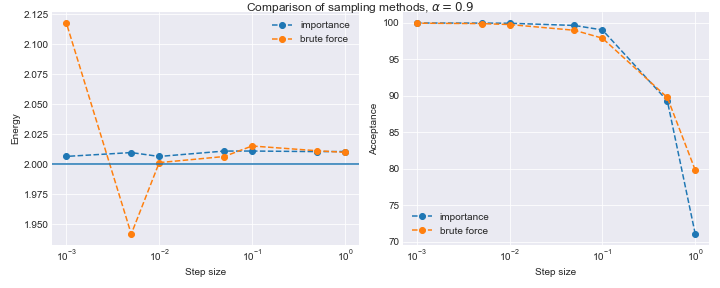
\includegraphics[width=\linewidth]{../Results/comparing_sampling}\caption{•}\label{fig:comparing_sampling}
\end{figure}

From the left part of the figure it can be observed that some of the expectation values for the energies are lower than the ground state energy ($dl = 0.005$ and $dl = 0.5$ for brute force sampling and importance sampling respectively) even though these calculations where done with $\alpha$ = 0.9. Furthermore, Tab. \ref{tab:importance_no_interaction_2p} compare the result of brute force sampling and importance sampling for different step sizes and include the SEM and $\sigma_b$. The numbers show that the SEM is underestimating the deviations and that including the correlations in the random number generator increases the deviation, giving us $\sigma_b$. However, neither the SEM or $\sigma_b$ seem indicate anything abnormal for the calculations resulting in the low expectation values for the energy. Therefore, I took a closer look at the actual local energies for the sampling methods.

\begin{table}[H]\caption{Comparing the results for importance/brute force sampling. Energy are in atomic units (a.u.) and CPU time is in units of seconds. Here the parameter $\alpha$ is set to 0.9 and number of MC cycles are 2$^{21}$.}\label{tab:importance_no_interaction_2p}
\begin{tabular}{l|l|l} 
 & Brute force: &  Importance:\\ \hline
\begin{tabular}{c} 
$dl$:\\ \hline
1.000\\
0.500\\
0.100\\
0.050\\
0.010\\
0.005\\
0.001\\
\end{tabular} & \begin{tabular}{ccccc}
 $\left< E_L \right>$: & SEM: & $\sigma_B$: & Acc.: & $t_{CPU}$:\\ \hline
2.011 & 0.00010 & 0.00068 & 79.834& 6.125\\
2.010 & 0.00010 & 0.00118 & 89.814& 5.812\\
2.013 & 0.00010 & 0.00496 & 97.951& 5.859\\
2.003 & 0.00010 & 0.00860 & 98.995& 5.656\\
2.004 & 0.00010 & 0.02281 & 99.798& 6.188\\
1.948 & 0.00004 & 0.01005 & 99.909& 6.359\\
2.018 & 0.00001 & 0.00211 & 99.980& 6.094\\ \hline
\end{tabular} & \begin{tabular}{ccccc}
$\left< E_L \right>$: & SEM: & $\sigma_B$: & Acc.: & $t_{CPU}$:\\ \hline
2.016 & 0.00012 & 0.00027 & 68.528& 8.453\\
1.987 & 0.00011 & 0.00026 & 82.230& 8.625\\
2.005 & 0.00011 & 0.00051 & 97.874& 8.203\\
2.012 & 0.00011 & 0.00070 & 99.358& 7.875\\
2.011 & 0.00010 & 0.00145 & 99.967& 7.984\\
2.011 & 0.00010 & 0.00214 & 99.992& 7.656\\
2.015 & 0.00011 & 0.00487 & 99.999& 7.703\\ \hline
\end{tabular}\\
& Mean CPU time: 6.01339 & Mean CPU time: 8.07143\\
\end{tabular}
\end{table}

Figure \ref{fig:brute_force_small_steps} shows how the energy is not stable for steps sizes smaller than 0.01, so even though the step sizes 0.001 and 0.01 seems to give reasonable expectation values for the energy (see Tab. \ref{tab:importance_no_interaction_2p} and Fig. \ref{fig:comparing_sampling}), Fig. \ref{fig:brute_force_small_steps} seems to show that that is sort of a lucky shot. I also saw this by running the calculation with brute force sampling and the step size, $0.005$, with different seeds for the random number generator. The expectation energy for five different runs where $\left< E_L \right>$ =  1.91487, 2.03452, 1.90805, 1.88356 and 1.9284. From Fig. \ref{fig:brute_force_larger_steps} one can observe that even $dl=0.1$ seems to be too small since it also reuslts in the local energy varying slowly and taking longer "trips" to higher energies and using many steps to get back down again, but for this step size the "trips" to higher energies are more frequent than for the smaller step sizes. I concluded that a step size of 0.5 is the best choice for the brute force sampling because it gives resonable changes of the local energy and an accpentance rate of $\sim$ 90 \%. 

\begin{figure}[H]
\begin{subfigure}{.5\textwidth}
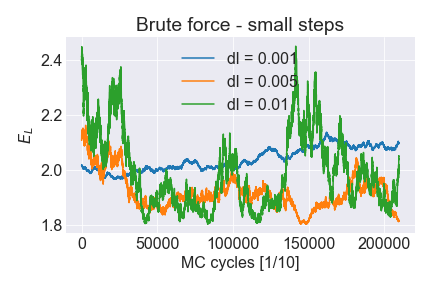
\includegraphics[width=\linewidth]{../Results/brute_force_small_steps}\caption{}\label{fig:brute_force_small_steps}
\end{subfigure}
\begin{subfigure}{.5\textwidth}
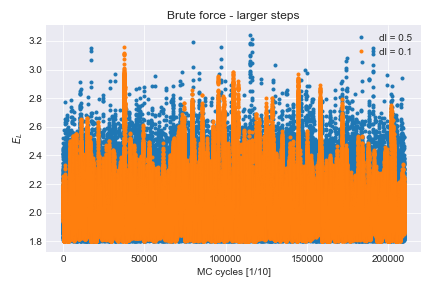
\includegraphics[width=\linewidth]{../Results/brute_force_larger_steps}\caption{}\label{fig:brute_force_larger_steps}
\end{subfigure}
\caption{•}\label{fig:brute_force_step_sizes}
\end{figure}

On the other hand, for the importance sampling, the investigation of the local energies did not give any clues to why the expecation energy is lower that the ground state energy for a step size of 0.5. Eventually I decided that the result itself indicate that 0.5 is a too large step size for importance sampling and taken together with a low acceptance rate at 0.5 ($\sim$ 82 \%) it is clear that a smaller step size is preferable. 

At last, it is interesting to note that the CPU time of importance sampling is higher than the brute force sampling, so even though brute force sampling has a lower acceptance rate, at the ideal step size, than importance sampling the two methods seems to be somewhat comparable at least for the system I am investigating.


\subsubsection{Including optimization}

Minimization rate of 0.5 seemed to be ideal. It resulted in the fewest steps until the parameter value stabilized both for guesses close to the optimal value and for guesses far away from the optimal value, but for the smallest trap frequencies I had to use $\gamma = $ 0.1 or 0.2. The parameters were optimized by trying out different first guesses for $\alpha$ and $\beta$ and tuning $\gamma$ so that the parameters stabilized during the first 200 iteretions. The optimal parameters were extracted from the mean of the last 50 iterations. An example run is shown in Fig. \ref{} for $\omega = 0.5$.

\subsubsection{Including interaction}

\begin{table}[H]\caption{Ground state energy of two interacting electrons in harmonic oscillator trap. Number of MC cycles are $2^{23}$}\label{tab:ground_state_energy_brute_force_interaction}
\center
\begin{tabular}{c|cccccrccc}
$\omega$ & $\alpha$ & $\beta$ & $\left< E_L \right>$ & SEM & $\sigma_B$ &  $\overline{r}_{12} \,\,\,$ & $\left< T \right>$  & $\left< V_{ext}\right>$ & $\left<V_{int} \right>$  \\ \hline
1.00000 & 0.98847 & 0.39965 & 3.0068 & 0.00001 & 0.00009 & 1.636 & 0.8944 & 1.2990 & 0.8135\\
0.50000 & 0.98061 & 0.31091 & 1.6674 & 0.00001 & 0.00010 & 2.481 & 0.4488 & 0.7051 & 0.5135\\
0.10000 & 0.94693 & 0.17764 & 0.4486 & 0.00001 & 0.00011 & 6.695 & 0.1003 & 0.1767 & 0.1716\\
0.05000 & 0.92747 & 0.13815 & 0.2609 & 0.00000 & 0.00011 & 10.389 & 0.0533 & 0.0997 & 0.1076\\
0.01000 & 0.88398 & 0.07287 & 0.0777 & 0.00000 & 0.00006 & 29.177 & 0.0129 & 0.0284 & 0.0364\\
\end{tabular}
\end{table}

\begin{table}[H]\caption{Ground state energy of two electrons in harmonic oscillator trap. Number of MC cycles are $2^{23}$}\label{tab:ground_state_energy_brute_force}
\center
\begin{tabular}{c|ccccc}
$\omega$ & $\alpha$ & $\left< E_L \right>$ & $\overline{r}_{12} $ & $\left< T \right>$  & $\left< V_{ext}\right>$ \\ \hline
1.00 & 1.0 & 2.00 & 0.885348 &  0.9965780 & 1.0034200 \\
0.50 & 1.0 & 1.00 & 1.252330 & 0.5018750 & 0.4981250 \\
0.10 & 1.0 & 0.20 & 2.783100 & 0.0993103 & 0.1006900 \\
0.05 & 1.0 & 0.10 & 3.882810 & 0.0506190 & 0.0493810 \\
0.01 & 1.0 & 0.02 & 9.018470 & 0.0099707 &  0.0100293 \\
\end{tabular}
\end{table}

\begin{table}[H]\caption{Ground state energy of two interacting electrons in harmonic oscillator trap. Number of MC cycles are $2^{22}$}\label{tab:ground_state_energy_importance_interaction}
\center
\begin{tabular}{c|ccccccccc}
$\omega$ & $\alpha$ & $\beta$ & $\left< E_L \right>$ & SEM & $\sigma_B$ & $|\bm{r}_1-\bm{r}_2|_{mean}$ & $\left< T \right>$  & $\left< V_{ext}\right>$ & $\left<V_{int} \right>$  \\ \hline
\end{tabular}
\end{table}

\subsection{One-body density}



\subsection{Extending to more particles}

\subsubsection{Six particles}

\subsubsection{Twelve particles}

